\section{State of the Art}

\subsection{On Affordances}

\subsubsection{The Concept of Affordances in HCI}

In Human-Computer Interaction (HCI), the term "affordance" plays a crucial role in understanding how users interact with interfaces,
 acting as a bridge between User Interface (UI) design and User Experience (UX).
 The concept of affordance refers to the properties or characteristics of an object (or a digital element) that indicate how it can be used, guiding users toward the appropriate action.
 It is a core principle that informs both the design of interfaces and the overall experience users have while interacting with a system.

Norman (1988) \cite{norman1988psychology} introduced the idea that affordances provide visual cues or hints about how an object should be used.
These cues help users understand an object’s function without needing instructions or labels.
For example, buttons in a user interface are designed to look clickable—whether through shading, placement, or labeling—immediately signaling to users that they should click or tap them to interact.
Norman emphasized that affordances are a blend of an object’s actual properties and the perceived suggestion of how it can be used.
In digital interfaces, this means that the design of an element communicates its function, such as sliders indicating adjustability or icons suggesting actions like saving or deleting.

This concept is deeply connected to the user experience because it shapes how easily and intuitively users can interact with an interface.
A well-designed UI should offer affordances that make the intended interactions clear, reducing the need for users to think about how to use the system. 
When the affordances of a design are clear, users can navigate and complete tasks with minimal friction, leading to a more seamless and satisfying UX.

Affordances also guide users by leveraging their existing mental models or prior experiences.
For example, users expect a trash can icon to afford the action of deleting because that is a widely understood visual metaphor.
The effectiveness of these affordances directly impacts the usability and the overall success of an interface, reinforcing the link between UI design and UX outcomes.

\begin{figure}[h]
    \centering
    
\includegraphics[width=\textwidth/3]{iconsAffordances.png}
    \caption{Functional icons indicate actions.}
    \vspace{0.1cm}
    \label{fig:affordances}
\end{figure}

Gibson’s (1977) \cite{gibson1977theory} perspective on affordances in the physical world also contributes to the HCI context.
Gibson viewed affordances as action possibilities inherent in an environment, regardless of whether the actor perceives them.
In the context of digital systems, this can translate to functionalities that exist within a user interface but might not be immediately visible or discoverable.
For instance, a hidden menu still has the affordance of being expandable, even if the user doesn't notice it initially.
However, the usability of a system greatly improves when affordances are both present and easily perceivable, which is where Norman’s concept ties back into the design of intuitive interfaces.

Affordances in HCI, therefore, are essential in making interfaces both functional and understandable.
They create a bridge between the UI, which consists of the visual elements and controls, and the UX, which is how users feel and perform when interacting with the system.
The more intuitive the affordances, the more positive the user experience, as users can operate the system effortlessly, feeling in control of the interface and its functionalities.

\subsubsection{ Affordances as the Link Between UI and UX}

The effectiveness of affordances directly influences the interaction between the user and the system.
In this way, affordances serve as a critical link between UI and UX, because they shape the user’s perception of how a system should function (UI) and ensure that the system behaves in a way that meets those expectations (UX).
 Poor affordances can lead to frustration or confusion, while clear affordances contribute to an intuitive, seamless user experience.
 For example, a button that visually appears pushable but doesn’t function as expected creates a disconnect between UI and UX, undermining trust in the system.

By incorporating affordances into UI design, designers ensure that users can interpret how to interact with the interface without needing to think about it.
 This predictability and ease of interaction enhance the overall user experience, making affordances a fundamental principle of successful HCI design.

Affordances are crucial in bridging the gap between UI and UX by providing users with clear, understandable cues for interaction, ensuring that digital systems are both usable and enjoyable to navigate.

\subsection{The Impact of Low Signaling but High Possibility Interfaces in HCI}

\subsubsection{Building on Affordances}

In the previous section, we explored the concept of affordances as a fundamental link between User Interface (UI) and User Experience (UX).
Affordances guide users through an interface by providing both actual and perceived cues about how an object or element can be interacted with.
When these affordances are clear, users can intuitively understand what actions are possible.
However, as digital interfaces evolve, particularly in the realms of augmented reality (AR) and artificial intelligence (AI), we encounter new types of interfaces where affordances are less explicit.
These \textbf{low-signaling, high-possibility} systems challenge traditional UI and UX paradigms, introducing new complexities in how users navigate and interact with the possibilities afforded by these systems.

\subsubsection{ Low Signaling, High Possibility Interfaces}

Low-signaling, high-possibility interfaces are characterized by the absence of clear visual or sensory cues that traditionally guide users in understanding how to interact with a system.
Despite offering a wide range of possible interactions and outcomes, these interfaces provide minimal affordances, making it difficult for users to easily discover the full scope of functionality.
This creates a disconnect between the vast potential of the system (high possibility) and the user's ability to perceive or act on that potential (low signaling).

For example, in an advanced digital system where gestures, voice commands, or implicit user behavior can trigger a variety of actions, the system may offer a high degree of interactivity.
However, without clear visual, auditory, or haptic cues to guide the user, it can be challenging to discern what actions are available or how to perform them.
This contrast between signaling levels and possibility levels highlights a critical design tension that impacts usability and user experience.

\subsubsection{ Signaling Levels vs. Possibility Levels}

To effectively design for both usability and richness in interaction, it's important to understand the balance between signaling levels and possibility levels:

\begin{itemize}
    \item \textbf{High Signaling, Low Possibility:} These interfaces are straightforward and easy to use, offering clear affordances for a limited range of actions. For instance, a simple media player might feature a play/pause button, volume controls, and a slider for adjusting the timeline—each with an obvious function.
    \item \textbf{Low Signaling, High Possibility:} These interfaces, by contrast, are complex, offering numerous interaction possibilities, but with minimal guidance or affordances. Voice command systems or gesture-based interfaces often fall into this category, where the user must experiment or learn to discover the breadth of possible interactions.
\end{itemize}
    
    

In many cases, increasing signaling—through visual or other sensory affordances—enhances the user's ability to explore the full potential of a system.
 However, in emerging fields like augmented reality (AR), increasing signaling can clutter the user's experience and overwhelm the interface, limiting the immersion that AR aims to create.

\subsection{ Augmented Reality (AR): High Possibility Limited by Signaling}

AR represents a prime example of the challenges posed by low-signaling, high-possibility interfaces.
In AR, the possibilities for interaction are vast—users can interact with digital objects overlaid onto the physical world in ways that blend virtual and real elements.
However, signaling these possibilities is often a challenge. AR environments are typically designed to be immersive, and designers must balance providing enough affordances to guide the user while avoiding excessive visual clutter that breaks the illusion of the physical-digital blend.

For example, an AR interface may allow users to manipulate virtual objects, trigger animations, or access additional information by performing gestures, using voice commands, or interacting with physical counterparts.
However, without clear affordances (such as icons, buttons, or animations), users may not know how to engage with these elements.
The high possibility for interaction is limited by the system's ability to communicate what those interactions are.

This limitation in AR emphasizes the need for innovative signaling techniques that do not overwhelm the user but still provide enough guidance to unlock the system's full interactive potential.
In traditional UIs, affordances are explicit; in AR, they must be more subtle, adaptive, and context-aware to maintain the immersive experience.

\subsubsection{ AI as an Enabler of High-Possibility, Low-Signaling Interfaces}

Artificial intelligence (AI) provides a powerful solution to the challenges posed by low-signaling, high-possibility interfaces.
AI-driven systems can analyze user behavior, interpret context, and dynamically provide interaction cues when needed, enabling a more fluid and intuitive experience in environments where visual or explicit affordances are minimal.

In low-signaling interfaces like voice assistants, for instance, AI allows users to interact with the system through natural language, reducing the need for explicit visual clues.
Similarly, in AR environments, AI can interpret a user's gaze, gestures, or contextual actions to offer subtle, on-the-fly guidance.
By dynamically adapting the interface to the user’s context, AI compensates for the lack of explicit affordances, enabling users to explore a wide range of possibilities without being overwhelmed by visual clutter.

\subsubsection{ AR and AI: A Symbiotic Solution to Signaling Challenges}

The integration of AI into AR represents a significant advancement in overcoming the signaling limitations of AR interfaces.
Together, AR and AI create a hybrid interaction model where AI interprets user intent and provides subtle, context-sensitive guidance, allowing AR environments to offer rich, high-possibility interactions without overwhelming the user with too many signals.

For example, AI can infer a user’s intent based on their actions and adaptively display affordances only when necessary—such as highlighting a virtual object when the user’s gaze rests on it or providing auditory feedback when a gesture is detected.
This dynamic signaling system enhances the user's ability to discover and use the full range of interactions available in AR, without disrupting the immersive nature of the experience.

By embedding AI into AR systems, designers can ensure that users are guided toward meaningful interactions, even in complex, high-possibility environments where traditional affordances might fail.
This combination not only compensates for the signaling limitations of AR but also unlocks new possibilities for how users engage with digital systems, creating more fluid, intuitive, and rewarding experiences.

\subsubsection{ Conclusion }

Low-signaling, high-possibility interfaces present unique challenges in HCI, particularly in AR environments where the richness of interaction is often limited by the ability to signal those possibilities to users.
However, AI introduces a transformative solution by enabling adaptive, context-sensitive guidance that compensates for the lack of explicit visual affordances.
As AR and AI converge, these technologies create interfaces that are not only immersive and rich in possibility but also intuitive and easy to navigate—bridging the gap between low-signaling and high-interaction environments.

By building on the foundation of affordances discussed in the previous chapter, this chapter highlights the evolving nature of interaction design, where AI-enhanced AR systems represent the next frontier of HCI.
These systems maintain the delicate balance between signaling and possibility, ensuring that users can fully engage with digital-physical environments without being constrained by the limitations of traditional affordance-based designs.

\subsection{ Detecting User Actions in AR}

\subsubsection{Introduction}

Accurate detection and interpretation of user actions are essential to creating immersive and responsive augmented reality (AR) applications.
Whether through gestures, facial expressions, or body movements, AR applications require robust mechanisms to interpret these actions in real time.
Two key technologies— \textbf{OpenPose} \cite{cao2017realtime} and \textbf{MediaPipe} \cite{lugaresi2019mediapipe} —enable this functionality, with \textbf{MediaPipe} emerging as the keystone framework for modern AR applications due to its efficiency and versatility, particularly for lightweight edge devices.
This chapter delves into how \textbf{MediaPipe} achieves 30 frames-per-second (FPS) body tracking on low-power devices, the optimizations made by Google, and the importance of dataset collection in making real-time interaction possible.

\begin{figure}[h]
    \centering
    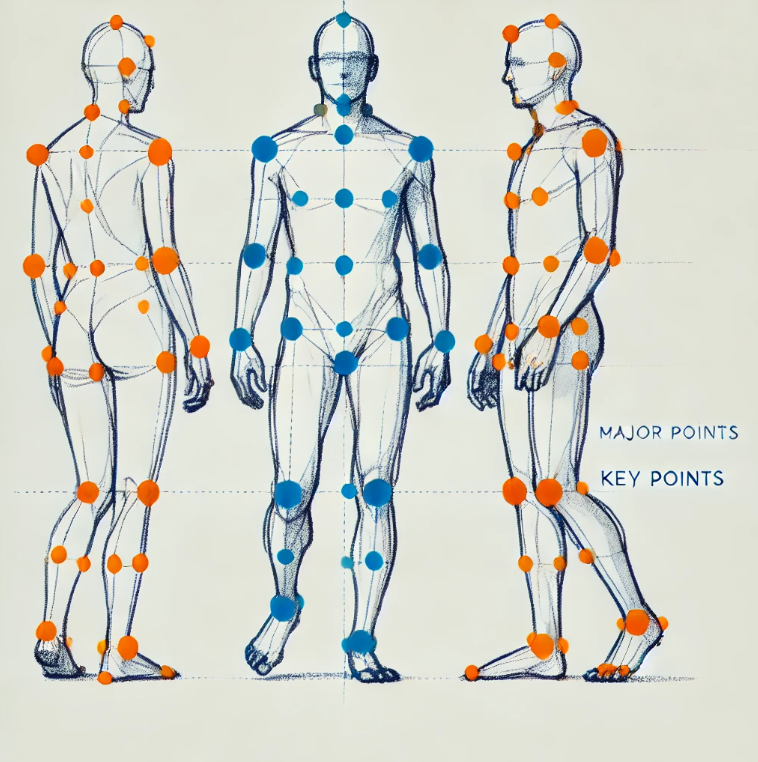
\includegraphics[width=\textwidth/3]{mediapipeKP.png}
    \caption{Simplified sketch showcasing keypoint tracking.}
    \vspace{0.1cm}
    \label{fig:kptracking}
\end{figure}

\subsubsection{ OpenPose: An Overview of Body Tracking}

Before exploring MediaPipe's strengths, it’s important to understand OpenPose, a widely used framework for detecting human body keypoints.
OpenPose tracks skeletal movements in real time, enabling AR systems to interpret user gestures and body movements by mapping them onto a digital model.
This technology allows AR applications to respond to the user’s physical actions, offering real-time feedback such as manipulating virtual objects or controlling an environment through gestures.
However, OpenPose's real-time tracking demands significant computational power, especially when handling multiple users or complex environments.
This makes it challenging to implement on mobile and edge devices, where hardware constraints limit processing capacity.

\subsubsection{ MediaPipe: Optimizing for Real-Time Tracking on Lightweight Devices}

\begin{figure}[h]
    \centering
    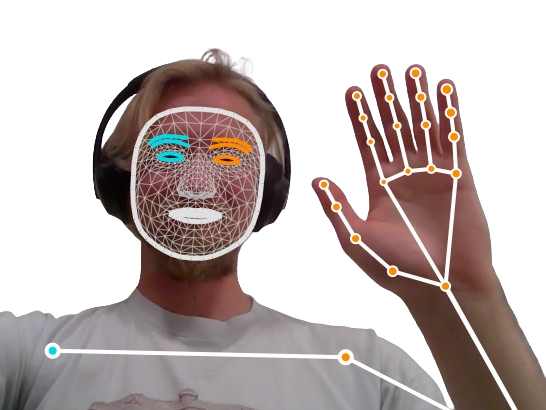
\includegraphics[width=\textwidth/2]{mediapipe.png}
    \caption{Key points tracked by mediapipe.}
    \vspace{0.1cm}
    \label{fig:mediapipe}
\end{figure}

While OpenPose excels at detailed body tracking, \textbf{MediaPipe} has become a game-changer for AR by enabling real-time body tracking at 30 FPS even on lightweight edge devices such as smartphones and AR glasses.
This real-time tracking is essential for creating smooth and responsive AR experiences, especially when users rely on immediate feedback from their gestures and movements.

Google’s work on \textbf{MediaPipe} involves significant optimizations to ensure that AR applications can run efficiently on devices with limited computational power, such as mobile phones.
The key to this optimization lies in both the model architecture and the extensive dataset collection and training undertaken by Google, which enables MediaPipe to balance accuracy, speed, and low resource consumption.

\subsubsection{ Model Optimization for Edge Devices}

MediaPipe's ability to deliver high-performance body tracking on lightweight devices is rooted in several core strategies:


\begin{itemize}
    \item \textbf{1. Efficient Model Architecture:} The neural networks powering MediaPipe are optimized for efficiency, focusing on reducing computational load without sacrificing accuracy. By designing compact model architectures, Google ensures that MediaPipe can perform complex inference tasks, such as pose estimation or facial landmark detection, with minimal latency. These models are designed to minimize floating-point operations (FLOPs), reducing the strain on device resources like memory and processing power.
    \item \textbf{2. Quantization:} One of the major optimizations employed in MediaPipe is the use of quantization techniques. In this process, model weights are reduced from 32-bit floating-point numbers to 8-bit integers, significantly reducing the size of the model and allowing it to run faster on hardware with limited capabilities. Quantized models maintain most of their accuracy while reducing both computation and memory requirements, making them ideal for real-time AR applications on edge devices.
    \item \textbf{3. Parallel Processing:} MediaPipe leverages the ability to run multiple inference models in parallel, utilizing the multicore architecture of modern devices. This ensures that body tracking, gesture recognition, and other processing tasks can be executed simultaneously, allowing the system to remain responsive even when handling complex inputs from various sensors, such as cameras and depth sensors.
    \item \textbf{4. Frame Skipping and Adaptive Inference:} MediaPipe can adaptively reduce the number of frames processed by dynamically skipping frames during periods of minimal movement. This adaptive inference technique saves processing power during less demanding phases while ensuring high responsiveness when movement is detected. This helps in maintaining smooth user experiences without taxing the device continuously.
    \item \textbf{5. Efficient Data Flow:} MediaPipe operates using a graph-based pipeline, where each computational step is treated as a node in a directed graph. This design allows data to flow efficiently between nodes, with each step of the tracking process being highly modular. This pipeline structure ensures minimal latency and optimizes the use of device resources, especially important in edge devices that process sensory data in real time.
\end{itemize}

\subsubsection{ Dataset Collection and Training}

Another cornerstone of MediaPipe’s success in real-time body tracking is the extensive and diverse dataset collection conducted by Google.
To ensure accurate body and gesture tracking, Google gathered large amounts of video and sensory data from diverse environments, including various lighting conditions, body types, and movement patterns.
This dataset forms the basis for training the machine learning models that power MediaPipe’s inference capabilities.

\begin{itemize}
    \item \textbf{1. Diverse Dataset:} To create robust body-tracking models, Google collected datasets that represented a wide range of human movements, facial expressions, and gestures across different demographics and environments. This diversity allows MediaPipe to maintain accuracy across different user profiles and ensures that AR applications can function reliably in different real-world scenarios.
    \item \textbf{2. Real-World Scenarios:} MediaPipe’s dataset was designed to reflect the challenges faced by AR applications in real-world settings. This includes training models on video streams with varying levels of occlusion, motion blur, and environmental noise. By incorporating these variables, MediaPipe ensures that its models can accurately track body movements even in suboptimal conditions, such as low-light environments or when the user’s body is partially obscured by other objects.
    \item \textbf{3. Transfer Learning:} MediaPipe leverages transfer learning to speed up the model training process. By using pre-trained models on general datasets and fine-tuning them with domain-specific data, MediaPipe can quickly adapt its models for AR applications without requiring vast computational resources or time for retraining.
\end{itemize}

\subsubsection{ MediaPipe: The Keystone for Modern AR Applications}

The result of these optimizations is that MediaPipe is now considered a foundational framework for modern AR applications, particularly those that run on edge devices.
Its ability to deliver 30 FPS real-time body tracking on mobile devices is a major breakthrough, enabling developers to build AR systems that are both highly interactive and efficient.

MediaPipe allows developers to create pipelines where user actions, such as gestures or facial expressions, are tracked and processed in real-time.
These actions can then trigger various AR experiences, from object manipulation to facial filters, with smooth transitions and minimal delay.
The combination of efficient model architecture, adaptive inference techniques, and a rich dataset allows MediaPipe to maintain high performance even in resource-constrained environments.

\subsubsection{ Conclusion}

Detecting user actions in AR is a critical component for building immersive, interactive experiences.
While OpenPose offers advanced capabilities for tracking user body movements, MediaPipe stands out as a highly optimized solution, particularly for lightweight edge devices.
Google's extensive work on model optimization, including techniques like quantization, adaptive inference, and parallel processing, enables MediaPipe to achieve real-time body tracking at 30 FPS on mobile devices.
Combined with its rich dataset collection, MediaPipe provides a robust platform for modern AR applications, making it an essential tool for developers working at the intersection of AR and AI. As AR continues to evolve, MediaPipe’s optimizations for resource efficiency and real-time processing will be key to enabling more complex and responsive user interactions in future applications.


\subsection{ The Evolution of Natural Language Processing in Machine Learning}

\subsubsection{ Introduction: From N-Grams to Modern Large Language Models (LLMs)}

Natural Language Processing (NLP) has undergone a remarkable evolution in the field of machine learning, from early techniques like N-grams \cite{Mar13} to the advent of modern large language models (LLMs).
Each milestone in this progression reflects the increasing complexity of language understanding and the growing sophistication of computational models designed to process human language.
Today, LLMs are not just powerful language processors; they have become semantic operators, revolutionizing how we interpret and interact with language. This section explores the evolution of NLP, highlights the rise of LLMs as semantic operators, and explains how these models are reshaping Human-Computer Interaction (HCI) by enabling interfaces with low affordance through low signaling and high possibility.

\subsubsection{ Early NLP: N-Grams and Statistical Models}

In the early stages of NLP, statistical models like \textbf{N-grams} were used to predict the likelihood of word sequences.
N-grams are based on the probability of a word occurring, given the previous N-1 words. For example, a bigram model predicts a word based on the one preceding it, while a trigram model uses the two preceding words. Though simple, N-grams were effective in tasks like speech recognition and text generation, offering a basic way to model language by counting word occurrences and calculating probabilities.

However, these models had significant limitations, especially when it came to understanding the broader context of language.
N-grams could only account for short-range dependencies and often struggled with ambiguity or meaning, as they were purely statistical and lacked deeper semantic understanding.
The reliance on limited context meant that these models could not effectively grasp the nuances of human language, prompting the development of more advanced techniques.

\subsubsection{ The Rise of Neural Networks and Word Embeddings}

The next significant leap in NLP came with the introduction of \textbf{neural networks} and \textbf{word embeddings}, particularly through models like Word2Vec \cite{rong2014word2vec} and GloVe\cite{pennington2014glove}.
Word embeddings transformed how machines interpreted language by mapping words to dense vectors that captured semantic relationships. This allowed words with similar meanings to have similar vector representations, enabling models to understand relationships like "king" is to "queen" as "man" is to "woman."

\begin{figure}[h]
    \centering
    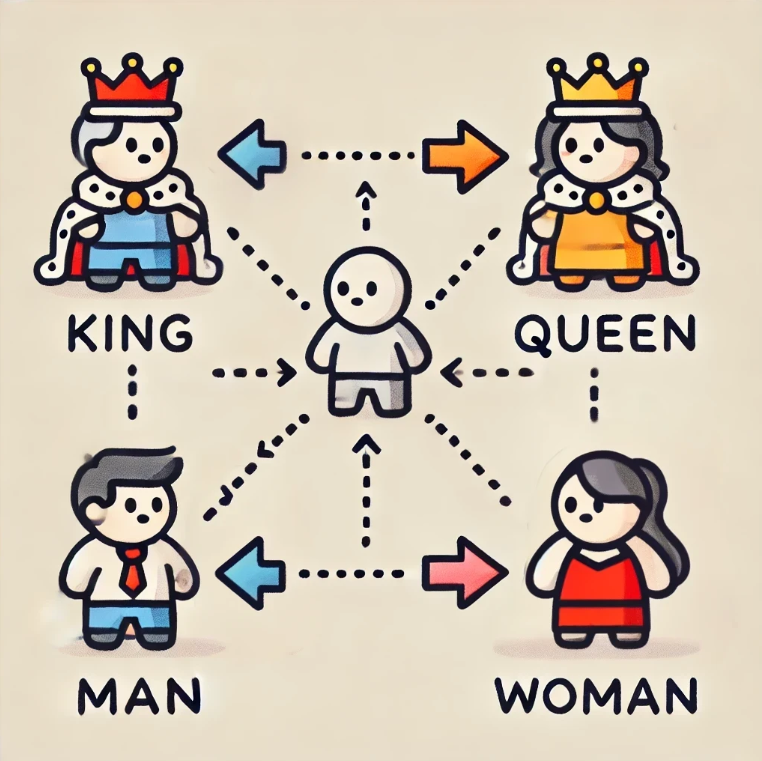
\includegraphics[width=\textwidth/3]{embedding.png}
    \caption{The mathematical operation that transforms the embedding of "man" to "woman" also transforms the embedding of "king" to "queen".}
    \vspace{0.1cm}
    \label{fig:embeddings}
\end{figure}

These embeddings, while a major step forward, still struggled with polysemy (words having multiple meanings) and couldn’t handle long-range dependencies well.
The need for a model that could understand context over entire sentences or paragraphs led to the development of \textbf{recurrent neural networks (RNNs)} \cite{Rumelhart1986LearningIR} and \textbf{long short-term memory (LSTM)} \cite{hochreiter1997long} networks, which improved the ability to capture sequential dependencies in language.

\subsubsection{ The Transformer Era and Large Language Models (LLMs)}

The breakthrough that brought NLP into the modern era was the development of the \textbf{Transformer} architecture, first introduced in the "Attention is All You Need" paper by Vaswani et al. in 2017 \cite{vaswani2017attention}. Unlike RNNs, Transformers rely entirely on a self-attention mechanism, allowing the model to focus on different parts of a sentence simultaneously, regardless of their position.
This enabled better handling of long-range dependencies and opened the door for scaling NLP models to unprecedented levels.

\begin{figure}[h]
    \centering
    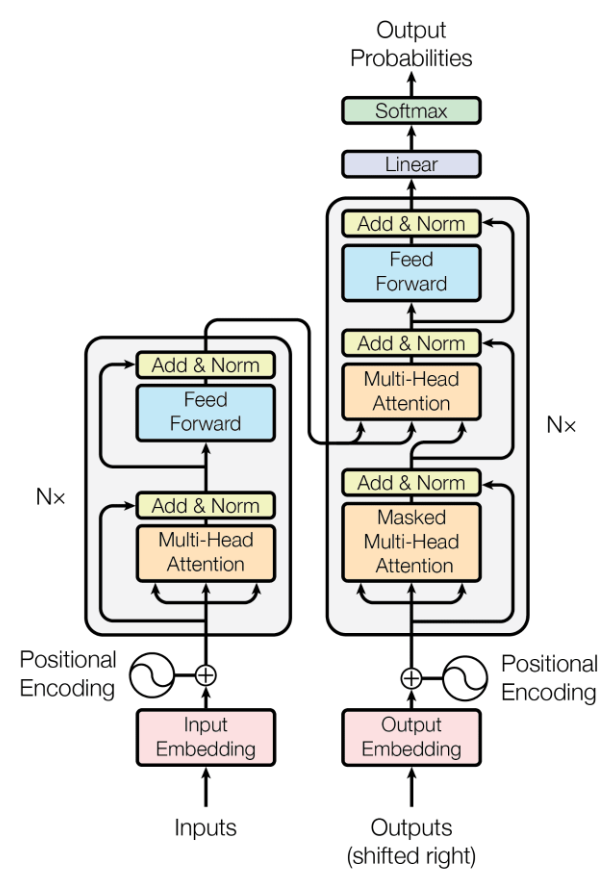
\includegraphics[width=\textwidth]{trasnformer.png}
    \caption{Overview of the Transformer architecture.}
    \vspace{0.1cm}
    \label{fig:transformer}
\end{figure}

Building on the Transformer architecture, \textbf{large language models (LLMs)} like \textbf{GPT (Generative Pre-trained Transformer)}\cite{radford2018improving} and \textbf{BERT (Bidirectional Encoder Representations from Transformers)}\cite{devlin2018bert} revolutionized NLP. LLMs trained on vast corpora of text have demonstrated the ability to perform tasks such as text generation, translation, summarization, and even answering complex questions.
These models don’t just analyze words—they understand context, intent, and meaning on a deep level, making them far more adept at processing human language.

The rise of Large Language Models (LLMs) marks a significant shift in accessibility and democratization of deep learning technologies.
Historically, large deep learning models required extensive computational resources and were primarily accessible to those with the expertise to manage complex architectures.
However, the introduction of \textbf{pay-as-you-go APIs} like ChatGPT and Claude, alongside open-source platforms like \textbf{Hugging Face}, has drastically lowered the barriers to entry.
These services enable developers to access and integrate powerful LLMs without the need for specialized infrastructure or deep expertise.
Now, even a simple microcontroller or edge device can leverage web APIs to tap into cutting-edge NLP capabilities, significantly reducing both development and maintenance costs.
This democratization has expanded the use of deep learning technologies, making them accessible to a broader audience across industries and enabling more innovation in human-computer interaction.

\subsubsection{ LLMs as Semantic Operators}

One of the most powerful aspects of modern LLMs is their function as \textbf{semantic operators}.
In computing, we are familiar with mathematical and logical operators, which are hardware-friendly and easily implemented.
However, \textbf{semantic operators}, which deal with meaning and interpretation, were traditionally reserved for the human domain.
With LLMs, machines can now function as semantic operators, interpreting, manipulating, and generating language in ways that reflect deeper understanding.

For example, when presented with the sentence "The cat sat on the mat," a mathematical model would simply process the syntax.
However, an LLM can infer more—understanding that "cat" is an animal, "sat" refers to the action of sitting, and "mat" is a surface.
More complex interpretations, like summarizing a paragraph or making inferences based on context, were historically exclusive to human cognition but are now within the domain of LLMs.

The ability of LLMs to act as semantic operators enables machines to comprehend and engage with the subtleties of language, making them invaluable for natural language tasks in HCI.
They allow systems to interact more naturally with users by understanding the meaning behind queries, interpreting ambiguous input, and even generating responses that align with human expectations.

\subsubsection{ Semantic Operators and Their Role in HCI}

In Human-Computer Interaction (HCI), semantic operators play a crucial role in designing interfaces that are more intuitive and responsive to user needs.
Traditionally, interfaces relied on explicit affordances—visual or physical cues that guide the user’s interaction with a system.
However, as we explored in previous sections, low-signaling, high-possibility interfaces challenge this paradigm by reducing the explicit affordances while increasing the range of possible interactions.

Here, LLMs as semantic operators become critical.
They allow systems to \textbf{infer user intent}, even when the signals provided by the interface are minimal or ambiguous.
For example, in a voice-activated system, the user may issue an incomplete or vague command, yet an LLM can interpret the context, predict intent, and generate an appropriate response.
This ability to operate with low signaling while maintaining high interaction possibilities creates a more flexible and powerful interface.

Semantic operators also enable interfaces to become more conversational, adaptive, and capable of handling ambiguous or context-dependent input, which is especially important in emerging technologies like \textbf{augmented reality (AR)} and \textbf{AI-driven interfaces}.
In these environments, where explicit affordances are often limited by the physical-digital blend, LLMs can act as the interpretative layer, allowing users to interact with complex systems through natural language or gestures, without needing predefined commands or explicit instructions.

\subsubsection{ Low Signaling, High Possibility Interfaces Powered by LLMs}

The combination of low signaling and high possibility interfaces, as discussed in the context of AR, finds its most effective solution in \textbf{LLM-driven interfaces}.
With LLMs functioning as semantic operators, users can interact with a system that offers numerous possibilities, but without overwhelming them with visual cues.
This is because LLMs excel at interpreting high-level instructions and adapting to context, providing dynamic feedback or actions based on minimal input from the user.

For instance, in an AR environment, a user might say, "Show me the nearest restaurant," without explicitly interacting with a visual affordance.
The system, powered by an LLM, would understand the intent behind the phrase, gather the relevant information, and present it to the user.
This is an example of how LLMs bridge the gap between \textbf{low-signaling interfaces}, where traditional affordances are sparse, and \textbf{high-possibility interfaces}, where many actions and outcomes are possible.

\subsubsection{ Conclusion}

The evolution of NLP from N-grams to modern LLMs has transformed how machines process, understand, and interact with human language.
LLMs, with their ability to function as semantic operators, have enabled machines to perform tasks once thought exclusive to human cognition, making them invaluable in HCI.
Their role in enabling \textbf{low-signaling, high-possibility interfaces} is particularly significant, as they allow users to interact with systems in a more natural, flexible, and intuitive way.
As LLMs continue to evolve, their impact on the future of HCI and natural language interfaces will only grow, offering new possibilities for seamless, intelligent interaction between humans and machines.